\section{Results}
\label{sec:results}

\subsection{The Submitted Results Are Explained by Data Leakage}
\label{sec:leak}
Table~\ref{tab:leak} reproduces the submitted protocol. Oversampling every discomfort grade to 5,243 samples before a 70/15/15 row split reproduces the submitted partition sizes exactly, and an untuned gradient-boosting classifier then reaches \LeakOldAcc\,\% accuracy, \LeakOldRecall\,\% recall and MCC \LeakOldMCC{}---numbers as high as those reported for E-DDQN in the submitted version, obtained without any reinforcement learning. Under that protocol \LeakDupPos{} of the \LeakTestPos{} positive test rows (\LeakDupPct\,\%) have an exact duplicate in the training split, and every session contributes to both splits. The unmodified submitted E-DDQN script behaves the same way: \OrigOldRecall\,\% recall and MCC \OrigOldMCC{} on the reconstructed partition, but MCC \OrigGrpMCC{} once the split respects session-linkage groups. With the same columns and a grouped split, gradient boosting falls to ROC-AUC \LeakGrpRocAuc{} (MCC \LeakGrpMCC{}). The published numbers therefore measure the ability to recognise duplicated and temporally adjacent samples of sessions seen during training, not the ability to detect cybersickness in new sessions. All results below use the leakage-free protocol of Section~\ref{sec:protocol}.

\begin{table*}[t]
\centering
\caption{Effect of the evaluation protocol on the same data (21 raw columns of the curated release). Test-split metrics; ``proxy'' marks the reconstruction of the submitted pipeline (its 41-feature files were not available).}
\label{tab:leak}
\resizebox{\textwidth}{!}{\begin{tabular}{llccccc}
\toprule
Model & Evaluation protocol & Acc. & Recall & Spec. & MCC & ROC-AUC \\
\midrule
HGB & Oversample to 5,243/grade, then 70/15/15 row split (submitted protocol) & 97.6 & 99.8 & 91.0 & 0.935 & 0.995 \\
HGB & Row-level random split, no oversampling & 95.3 & 94.1 & 96.3 & 0.905 & 0.992 \\
HGB & Grouped 5-fold split (session-linkage groups) & 52.2 & 33.6 & 66.9 & 0.005 & 0.523 \\
E-DDQN (submitted code) & Submitted script, submitted protocol (proxy) & 95.2 & 99.2 & 83.1 & 0.870 & -- \\
E-DDQN (submitted code) & Submitted script, grouped split (proxy) & 41.1 & 92.1 & 7.7 & $-$0.004 & -- \\
\bottomrule
\end{tabular}
}
\end{table*}

\subsection{Leakage-Free Comparison under the 5:1 Cost}
\label{sec:main}
Table~\ref{tab:main} reports the primary analysis: every model tuned, checkpointed and thresholded on validation groups only and scored once on the outer-test groups (all \nSamplesEval{} samples, \nSessionsEval{} sessions). Two facts dominate. First, the detection problem is hard once sessions and participants are not shared: the best ranking performance is ROC-AUC \HGBCostRocAucMean{} (HGB) and \RFCostRocAucMean{} (random forest), and the highest mean PR-AUC is \DQNCostPrAucMean{} (DQN) against a prevalence of 0.44. Second, under a 5:1 cost the cost-minimising operating point of every model lies close to ``always alarm'' (cost \AlwaysCost): validation-selected thresholds yield recall of 93--99\,\% but specificity of only 3--18\,\%. Only the random forest improves materially on the trivial policy (cost \RFCostCostMean$\pm$\RFCostCostSD{} vs.\ \AlwaysCost), and even its group-bootstrap 95\,\% CI (seed ensemble, \RFCICostLo--\RFCICostHi) includes the always-alarm cost; logistic regression (\LRCostCostMean) and gradient boosting (\HGBCostCostMean) improve on it only marginally.

The corrected E-DDQN ranks last of the \nModels{} models on the primary rule: recall \EDDQNCostRecallMean$\pm$\EDDQNCostRecallSD\,\%, specificity \EDDQNCostSpecMean$\pm$\EDDQNCostSpecSD\,\%, cost \EDDQNCostCostMean$\pm$\EDDQNCostCostSD{} (worse than always alarming), ROC-AUC \EDDQNCostRocAucMean$\pm$\EDDQNCostRocAucSD{} and MCC \EDDQNCostMCCMean. The standard DQN baseline reaches cost \DQNCostCostMean{} and ROC-AUC \DQNCostRocAucMean, and the contextual-bandit variant E-CB cost \ECBCostCostMean{} and ROC-AUC \ECBCostRocAucMean. Neither RL model beats the cost of always alarming. E-DDQN therefore does \emph{not} improve on the standard DQN in this controlled comparison; the improvement reported in the submitted version does not survive leakage-free evaluation.

\begin{table*}[t]
\centering
\caption{Primary analysis (rule D1: threshold minimising the 5:1 cost on pooled inner-validation predictions). Mean~$\pm$~SD over five seeds of the pooled outer-test metrics (\nSamplesEval{} samples; recall, specificity, precision, F1 and balanced accuracy in \%); FN and FP are exact counts of the seed ensemble. Bold: lowest cost. HGB and logistic regression are deterministic given the data, hence SD = 0.}
\label{tab:main}
\resizebox{\textwidth}{!}{\begin{tabular}{lccccccccccc}
\toprule
Model & Recall & Spec. & Prec. & F1 & Bal. acc. & MCC & Cost$_{5:1}$ & ROC-AUC & PR-AUC & FN & FP \\
\midrule
\textbf{E-DDQN} & 93.4$\pm$2.5 & 7.4$\pm$2.7 & 44.4$\pm$0.7 & 60.2$\pm$0.9 & 50.4$\pm$1.2 & 0.016$\pm$0.054 & 0.663$\pm$0.048 & 0.538$\pm$0.016 & 0.483$\pm$0.019 & 400 & 4,820 \\
E-CB & 97.1$\pm$2.9 & 8.4$\pm$2.8 & 45.6$\pm$0.6 & 62.1$\pm$1.0 & 52.8$\pm$1.2 & 0.122$\pm$0.052 & 0.575$\pm$0.055 & 0.653$\pm$0.011 & 0.562$\pm$0.006 & 140 & 4,480 \\
DQN & 95.2$\pm$2.7 & 14.5$\pm$4.9 & 46.8$\pm$1.0 & 62.8$\pm$0.8 & 54.8$\pm$1.6 & 0.158$\pm$0.038 & 0.584$\pm$0.040 & 0.661$\pm$0.013 & 0.595$\pm$0.022 & 129 & 4,391 \\
CS-MLP & 99.4$\pm$0.7 & 2.8$\pm$1.9 & 44.7$\pm$0.4 & 61.7$\pm$0.4 & 51.1$\pm$0.8 & 0.072$\pm$0.049 & 0.557$\pm$0.012 & 0.644$\pm$0.018 & 0.521$\pm$0.022 & 23 & 4,925 \\
LogReg & 99.1$\pm$0.0 & 8.1$\pm$0.0 & 46.0$\pm$0.0 & 62.9$\pm$0.0 & 53.6$\pm$0.0 & 0.167$\pm$0.000 & 0.532$\pm$0.000 & 0.626$\pm$0.000 & 0.576$\pm$0.000 & 36 & 4,817 \\
HGB & 97.0$\pm$0.0 & 14.6$\pm$0.0 & 47.3$\pm$0.0 & 63.6$\pm$0.0 & 55.8$\pm$0.0 & 0.197$\pm$0.000 & 0.543$\pm$0.000 & 0.692$\pm$0.000 & 0.593$\pm$0.000 & 124 & 4,479 \\
RF & 98.5$\pm$0.3 & 18.2$\pm$0.7 & 48.8$\pm$0.2 & 65.2$\pm$0.1 & 58.3$\pm$0.3 & 0.266$\pm$0.004 & \textbf{0.491$\pm$0.003} & 0.688$\pm$0.002 & 0.548$\pm$0.001 & 54 & 4,281 \\
\midrule
Always alarm & 100.0 & 0.0 & 44.2 & 61.3 & 50.0 & 0.000 & 0.558 & -- & -- & 0 & 5,243 \\
Never alarm & 0.0 & 100.0 & -- & -- & 50.0 & 0.000 & 2.208 & -- & -- & 4,147 & 0 \\
\bottomrule
\end{tabular}
}
\end{table*}

\begin{figure}[t]
\centering
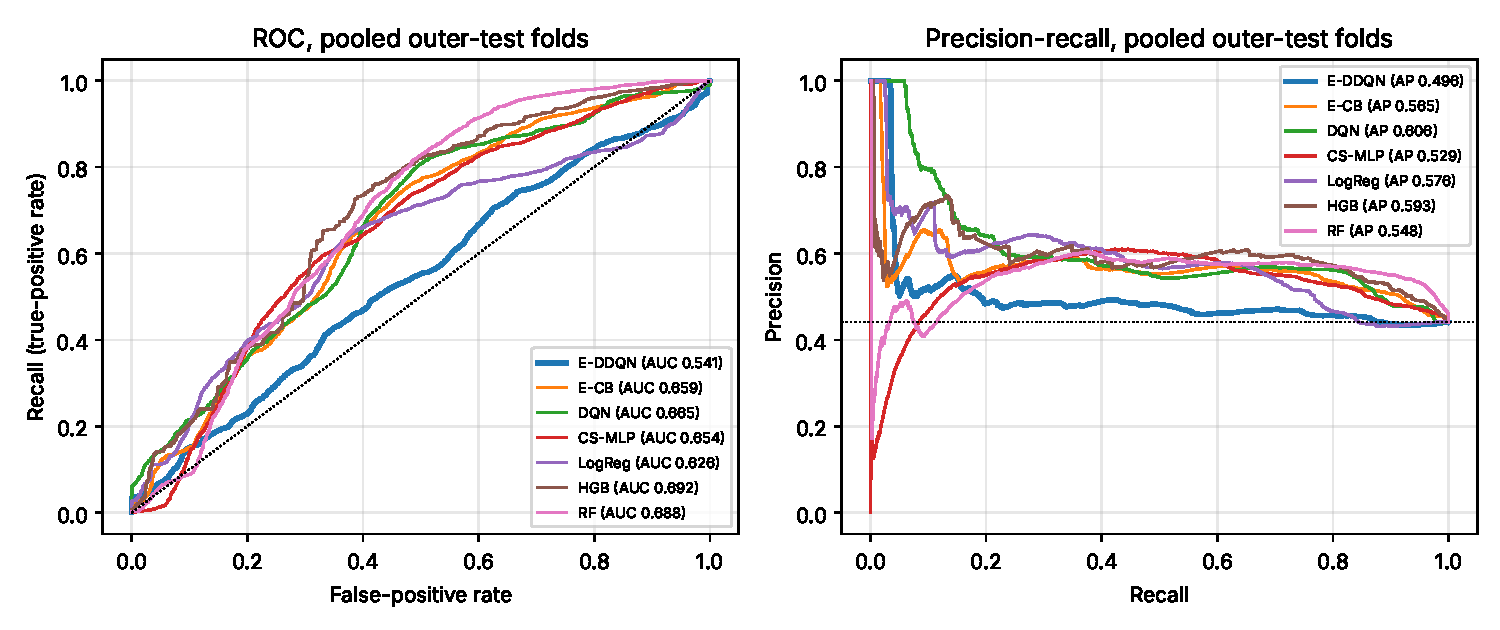
\includegraphics[width=\columnwidth]{figs/roc_pr_main.pdf}
\caption{ROC and precision--recall curves of the seed-ensemble scores, pooled over the five outer-test folds.}
\label{fig:rocpr}
\end{figure}

\subsection{Operating Points, Matched Recall and the Asymmetric Reward}
\label{sec:op}
Table~\ref{tab:ops} contrasts three operating rules. With the untuned Bayes cut-off $\hat p\ge 1/6$ (rule D0)---for the asymmetric agents this is simply the greedy policy $\arg\max_a Q(s,a)$---E-DDQN obtains recall \EDDQNBayesRecallMean\,\% at specificity \EDDQNBayesSpecMean\,\% (cost \EDDQNBayesCostMean), whereas the random forest obtains recall \RFBayesRecallMean\,\% at specificity \RFBayesSpecMean\,\% (cost \RFBayesCostMean). When every model is held to a validation recall of at least 0.95, the random forest again has the lowest cost (\RFRecCostMean; E-DDQN \EDDQNRecCostMean). At validation-matched recall targets (Table~\ref{tab:matched}), the thresholds transfer worst for E-DDQN: at both recall targets it attains lower test recall than every supervised model, and at the 0.95 target it also has a higher false-positive rate than all of them. Reading the ROC curves at fixed recall (descriptive only), the false-positive rate at 95\,\% recall is \EDDQNRocFPRatNineFive\,\% for E-DDQN and \RFRocFPRatNineFive\,\% for the random forest. Because the reward encodes the same 5:1 operating point as a cost-weighted classifier (Eq.~\eqref{eq:margin}), the asymmetric reward provides no advantage that cost-weighted training plus a validation-selected threshold does not already provide.

\begin{table}[t]
\centering
\caption{Expected 5:1 cost (mean over seeds) under three operating rules chosen without test data.}
\label{tab:ops}
\footnotesize
\begin{tabular}{lccc}
\toprule
Model & D1: min cost & D0: $\hat p\ge 1/6$ & val.\ recall $\ge$ 0.95 \\
\midrule
E-DDQN & \EDDQNCostCostMean & \EDDQNBayesCostMean & \EDDQNRecCostMean \\
E-CB & \ECBCostCostMean & \ECBBayesCostMean & \ECBRecCostMean \\
DQN & \DQNCostCostMean & \DQNBayesCostMean & \DQNRecCostMean \\
CS-MLP & \CSMLPCostCostMean & \CSMLPBayesCostMean & \CSMLPRecCostMean \\
LogReg & \LRCostCostMean & \LRBayesCostMean & \LRRecCostMean \\
HGB & \HGBCostCostMean & \HGBBayesCostMean & \HGBRecCostMean \\
RF & \RFCostCostMean & \RFBayesCostMean & \RFRecCostMean \\
\midrule
Always alarm & \AlwaysCost & \AlwaysCost & \AlwaysCost \\
\bottomrule
\end{tabular}
\end{table}

\begin{table*}[t]
\centering
\caption{Matched operating points: thresholds chosen on validation predictions to reach the stated recall or specificity; test recall (\%), false-positive rate (\%) and false-positive count of the seed ensemble.}
\label{tab:matched}
\resizebox{\textwidth}{!}{\begin{tabular}{lccccccccc}
\toprule
 & \multicolumn{3}{c}{val. recall $\ge$ 0.90} & \multicolumn{3}{c}{val. recall $\ge$ 0.95} & \multicolumn{3}{c}{val. specificity $\ge$ 0.80} \\
Model & Rec. & FPR & FP & Rec. & FPR & FP & Rec. & FPR & FP \\
\midrule
E-DDQN & 81.7 & 77.0 & 4,036 & 84.5 & 86.6 & 4,539 & 25.2 & 18.6 & 974 \\
E-CB & 88.6 & 68.0 & 3,565 & 92.4 & 78.1 & 4,093 & 31.2 & 17.4 & 910 \\
DQN & 88.0 & 64.2 & 3,366 & 91.7 & 72.7 & 3,810 & 32.2 & 14.2 & 743 \\
CS-MLP & 94.1 & 78.4 & 4,111 & 97.5 & 85.1 & 4,463 & 24.2 & 12.7 & 666 \\
LogReg & 92.8 & 73.5 & 3,856 & 97.2 & 81.7 & 4,285 & 37.7 & 22.5 & 1,181 \\
HGB & 95.4 & 72.2 & 3,785 & 97.5 & 81.7 & 4,282 & 24.3 & 11.3 & 594 \\
RF & 93.7 & 64.0 & 3,358 & 96.9 & 74.3 & 3,896 & 21.0 & 13.3 & 695 \\
\bottomrule
\end{tabular}
}
\end{table*}

\subsection{Statistical Comparison}
\label{sec:stats}
Table~\ref{tab:paired} compares E-DDQN with every other model on identical test samples (seed ensembles, rule D1). For every pair the McNemar contingency table satisfies $b-c=\mathrm{err}_B-\mathrm{err}_A$ (checked programmatically and recomputed with an independent library). Sample-level McNemar tests give $p<0.001$ for every pair, but they treat \nSamplesEval{} strongly autocorrelated seconds as independent and overstate the evidence. The group bootstrap, which resamples the \nGroupsEval{} independent units, shows that E-DDQN's cost is higher than that of the random forest by \PairDOneRFCostDiff{} (95\,\% CI \PairDOneRFCostLo{} to \PairDOneRFCostHi; $p=$\,\PairDOneRFPboot), higher than gradient boosting by \PairDOneHGBCostDiff{} ($p=$\,\PairDOneHGBPboot), logistic regression by \PairDOneLRCostDiff{} ($p=$\,\PairDOneLRPboot), CS-MLP by \PairDOneCSMLPCostDiff{} ($p=$\,\PairDOneCSMLPPboot) and E-CB by \PairDOneECBCostDiff{} ($p=$\,\PairDOneECBPboot); the difference from the standard DQN (\PairDOneDQNCostDiff; $p=$\,\PairDOneDQNPboot) is not significant at the 5\,\% level. Group-bootstrap confidence intervals of every model are given in Supplementary Sec.~S3.2; with only \nGroupsEval{} independent groups they are wide.

\begin{table*}[t]
\centering
\caption{Paired comparisons with E-DDQN (A) on the same \nSamplesEval{} test samples (seed ensembles, rule D1). $b$: A correct, B wrong; $c$: A wrong, B correct. $\Delta$Cost and its CI and $p_{\text{group}}$ come from 2,000 group-bootstrap replicates; $p_{\text{exact}}$ is the sample-level exact McNemar test.}
\label{tab:paired}
\resizebox{\textwidth}{!}{\begin{tabular}{lcccccccc}
\toprule
B (vs. A = E-DDQN) & $b$ & $c$ & err$_A$ & err$_B$ & $\chi^2_{cc}$ & $p_{\text{exact}}$ & $\Delta$Cost$_{5:1}$ (A$-$B) [95\% CI] & $p_{\text{group}}$ \\
\midrule
E-CB & 299 & 899 & 5,220 & 4,620 & 299.5 & $<$0.001 & +0.175 [+0.016, +0.448] & 0.014 \\
DQN & 297 & 997 & 5,220 & 4,520 & 377.6 & $<$0.001 & +0.190 [$-$0.017, +0.493] & 0.079 \\
CS-MLP & 402 & 674 & 5,220 & 4,948 & 68.3 & $<$0.001 & +0.190 [+0.005, +0.485] & 0.039 \\
LogReg & 389 & 756 & 5,220 & 4,853 & 117.0 & $<$0.001 & +0.194 [+0.011, +0.477] & 0.026 \\
HGB & 203 & 820 & 5,220 & 4,603 & 370.9 & $<$0.001 & +0.183 [+0.011, +0.460] & 0.035 \\
RF & 293 & 1,178 & 5,220 & 4,335 & 531.2 & $<$0.001 & +0.242 [+0.052, +0.528] & 0.001 \\
\bottomrule
\end{tabular}
}
\end{table*}

\subsection{Event-Level Behaviour}
At the cost-optimal operating points every model flags almost every session: E-DDQN raises an alarm on \EDDQNEvFreeAlarm\,\% of the seconds of the \nEventFreeSessions{} sessions in which no discomfort was ever reported and on \EDDQNEvPreAlarm\,\% of the seconds before onset in the \nEventSessions{} sessions with an event (random forest: \RFEvFreeAlarm\,\% and \RFEvPreAlarm\,\%). Events are therefore ``detected'' with zero median delay by construction, not through discrimination (Supplementary Sec.~S3.4).

\subsection{Why E-DDQN Under-Performs: Bootstrapping and Selection Optimism}
\label{sec:why}
Validation selected $\gamma=$ \EDDQNGammas{} for the five outer folds of E-DDQN, i.e.\ strong bootstrapping, and the exposure+profile feature set in \EDDQNnProfile{} of 5 folds. Section~\ref{sec:formulation} shows that bootstrapping cannot improve the optimal policy here and adds action-independent estimation noise to $\Delta Q$. Two diagnostics agree. (i) The separately tuned $\gamma=0$ variant (E-CB) ranks much better (ROC-AUC \ECBCostRocAucMean{} vs.\ \EDDQNCostRocAucMean). (ii) Table~\ref{tab:optimism} compares, per family, the inner-validation cost of the configuration at the moment it was selected with its outer-test cost. The gap is \EDDQNOptGap{} for E-DDQN but between \RFOptGap{} and \ECBOptGap{} for all other models: noisy, high-variance training curves combined with validation checkpointing and selection let E-DDQN configurations look best on validation folds by chance~\cite{varma2006bias}. Q-value estimates stay finite---the largest magnitudes over all runs (E-DDQN \EDDQNQAbsMax, DQN \DQNQAbsMax, E-CB \ECBQAbsMax) slightly exceed the corresponding return bounds $r_{\max}/(1-\gamma)$ in a few runs, i.e.\ extrapolation on atypical states---so the failure is not numerical divergence; the mean greedy-action Q-value differs from its realised discounted validation return by \EDDQNOverest{} for E-DDQN, \DQNOverest{} for DQN and \ECBOverest{} for E-CB (Supplementary Sec.~S3.6).

\begin{table}[t]
\centering
\caption{Selection optimism: pooled inner-validation 5:1 cost of the selected configuration (HPO seed) versus its outer-test cost (mean over folds and seeds).}
\label{tab:optimism}
\resizebox{\columnwidth}{!}{\begin{tabular}{lccc}
\toprule
Model & Inner-OOF cost at selection & Outer-test cost & Gap \\
\midrule
E-DDQN & 0.467 & 0.754 & +0.288 \\
E-CB & 0.488 & 0.557 & +0.070 \\
DQN & 0.478 & 0.544 & +0.065 \\
CS-MLP & 0.501 & 0.534 & +0.033 \\
LogReg & 0.518 & 0.531 & +0.014 \\
HGB & 0.518 & 0.539 & +0.021 \\
RF & 0.495 & 0.481 & $-$0.015 \\
\bottomrule
\end{tabular}
}
\end{table}

\subsection{Component Ablation and Reward-Ratio Sensitivity}
\label{sec:ablation}
Table~\ref{tab:ablation} removes or changes one component of E-DDQN at a time while keeping the configuration selected for each outer fold fixed (five seeds; same protocol). Every variant ranks close to chance (ROC-AUC \AblSoftCostRocAuc--\AblGammaZeroCostRocAuc). No single change moves the cost by more than about one seed standard deviation of the full model (\EDDQNCostCostMean$\pm$\EDDQNCostCostSD). The lowest cost is obtained by \emph{replacing} the asymmetric reward with the symmetric $\pm1$ reward (\AblAsymCostCost) and the highest ROC-AUC by switching off bootstrapping ($\gamma=0$; \AblGammaZeroCostRocAuc); hard target copies (\AblSoftCostCost), no dueling head (\AblDuelCostCost), uniform replay (\AblBalCostCost), no warm-up (\AblWarmCostCost) and toggling full-information replay (\AblFullCostCost) leave the cost essentially unchanged, and removing the double estimator slightly increases it (\AblDoubleCostCost). In contrast to the ablation of the submitted version, none of these components can be credited with a gain in safety or accuracy. Every variant is scored on the same implied-probability scale and thresholded with the same rules, so the reward table can act only through the learned scores; at the fixed cut-off $\hat p\ge1/6$ (rule D0) the symmetric-reward variant is not worse either (cost \AblAsymBayesCost{} vs.\ \EDDQNBayesCostMean).

\begin{table}[t]
\centering
\caption{Leave-one-component-out ablation of E-DDQN (selected configuration per outer fold held fixed; rule D1; mean over 5 seeds, cost $\pm$ SD).}
\label{tab:ablation}
\resizebox{\columnwidth}{!}{\begin{tabular}{lccccc}
\toprule
Variant & Recall & Spec. & Cost$_{5:1}$ & ROC-AUC & PR-AUC \\
\midrule
Full E-DDQN (selected) & 93.4 & 7.4 & 0.663$\pm$0.048 & 0.538 & 0.483 \\
\midrule
full-information replay toggled & 93.7 & 5.4 & 0.667$\pm$0.106 & 0.563 & 0.500 \\
symmetric $\pm$1 reward instead of asymmetric & 94.8 & 8.6 & 0.625$\pm$0.038 & 0.572 & 0.517 \\
uniform instead of class-balanced replay & 94.3 & 4.3 & 0.660$\pm$0.045 & 0.554 & 0.486 \\
no double estimator (max-operator target) & 93.1 & 5.3 & 0.681$\pm$0.086 & 0.543 & 0.491 \\
no dueling head & 94.6 & 5.8 & 0.644$\pm$0.059 & 0.559 & 0.494 \\
hard target copy every 10 updates & 94.9 & 6.5 & 0.634$\pm$0.043 & 0.529 & 0.472 \\
no warm-up & 93.8 & 7.1 & 0.656$\pm$0.049 & 0.547 & 0.497 \\
$\gamma=0$ (contextual bandit) & 94.4 & 6.4 & 0.645$\pm$0.070 & 0.576 & 0.510 \\
\bottomrule
\end{tabular}
}
\end{table}

Table~\ref{tab:ratio} varies the false-negative to false-positive regret of the reward from 1:1 to 10:1 (E-DDQN configuration per fold fixed; ratio 5:1 reproduces the main E-DDQN run bit for bit, which also confirms the determinism of the pipeline). The greedy policy moves along the trade-off exactly as Eq.~\eqref{eq:margin} predicts: recall rises from \RatioArgOneRecall\,\% (1:1) to \RatioArgFiveRecall\,\% (5:1) and \RatioArgOneZeroRecall\,\% (10:1), while specificity falls from \RatioArgOneSpec\,\% to \RatioArgFiveSpec\,\% and \RatioArgOneZeroSpec\,\%. Once the threshold is chosen on validation data, however, all ratios end at statistically indistinguishable costs (\RatioTunedOneCost--\RatioTunedOneZeroCost) and similar ranking: the reward ratio sets the default operating point, but it does not create discrimination that a threshold cannot reproduce. The 5:1 ratio is therefore best understood as a declared safety preference whose operating point can equally be reached by cost-weighted training or threshold selection.

\begin{table*}[t]
\centering
\caption{Reward-ratio sensitivity of E-DDQN: operating point of the greedy (arg-max) policy, whose implied cut-off on $P(y=1\mid s)$ is $1/(1+R)$, and of the validation-tuned threshold (rule D1). Mean ($\pm$ SD) over five seeds.}
\label{tab:ratio}
\footnotesize
\begin{tabular}{lcccccccc}
\toprule
 & & \multicolumn{3}{c}{Greedy policy ($\arg\max_a Q$)} & \multicolumn{3}{c}{Validation-tuned threshold (D1)} & \\
FN:FP regret & implied cut-off & Recall & Spec. & Cost$_{5:1}$ & Recall & Spec. & Cost$_{5:1}$ & ROC-AUC \\
\midrule
1:1 & $1/2$ & 52.4$\pm$5.6 & 58.1$\pm$4.8 & 1.285 & 94.9 & 7.4 & 0.629$\pm$0.056 & 0.558 \\
2:1 & $1/3$ & 69.2$\pm$3.3 & 43.1$\pm$1.6 & 0.999 & 94.6 & 6.4 & 0.642$\pm$0.074 & 0.563 \\
5:1 & $1/6$ & 77.2$\pm$3.8 & 28.0$\pm$2.0 & 0.905 & 93.4 & 7.4 & 0.663$\pm$0.048 & 0.538 \\
10:1 & $1/11$ & 80.7$\pm$3.2 & 23.0$\pm$3.3 & 0.855 & 92.9 & 7.4 & 0.673$\pm$0.095 & 0.552 \\
\bottomrule
\end{tabular}

\end{table*}



\subsection{Robustness under Telemetry Perturbations}
\label{sec:attack}
Table~\ref{tab:attack-auc} reports threshold-free ranking performance under each frozen perturbation. \AttAucFracSmall\,\% of the model--scenario combinations change the pooled ROC-AUC by less than 0.03 and none by more than \AttAucMaxAbsChange{} (the largest drops occur for acceleration-spike injection in E-CB and DQN and for speed down-scaling in gradient boosting), and several perturbations even raise it slightly: the detectors depend only weakly on the frame-rate, orientation and locomotion channels, mainly because the dominant inputs selected on validation data are exposure time, cumulative exposure and questionnaire answers. At the cost-optimal operating points (Table~\ref{tab:attack}), the per-session worst-case evasion adversary lowers recall on event seconds from \EDDQNAttCleanRecall\,\% to \EDDQNAttWorstRecall\,\% for E-DDQN, from \ECBAttCleanRecall\,\% to \ECBAttWorstRecall\,\% for E-CB and from \RFAttCleanRecall\,\% to \RFAttWorstRecall\,\% for the random forest, while the false-alarm adversary drives the false-positive rate of every model to \EDDQNAttWorstFPR--100\,\% (it is already \RFAttCleanFPR--\CSMLPAttCleanFPR\,\% without attack). These are feature-space stress tests: they show how far bounded manipulation of the logged channels can move the detectors' decisions, not what a real rendering attack would do to a participant, and they cannot evaluate field-of-view manipulation, which never varies in the data.

\begin{table*}[t]
\centering
\caption{Threshold-free robustness: pooled outer-test ROC-AUC of the seed-ensemble score on clean telemetry and under whole-session perturbations (the last column gives the most negative and most positive change over all 21 whole-session variants).}
\label{tab:attack-auc}
\resizebox{\textwidth}{!}{\begin{tabular}{lcccccccc}
\toprule
Model & Clean & fps$\le$45 & jitter 0.10 & speed $\times$1.5 & spikes 40 & speed $\times$0.5 & smooth 0.25 & min / max $\Delta$ \\
\midrule
E-DDQN & 0.541 & 0.541 & 0.593 & 0.561 & 0.559 & 0.532 & 0.539 & $-$0.008 / +0.053 \\
E-CB & 0.659 & 0.659 & 0.682 & 0.648 & 0.575 & 0.648 & 0.658 & $-$0.089 / +0.052 \\
DQN & 0.665 & 0.665 & 0.677 & 0.680 & 0.605 & 0.632 & 0.676 & $-$0.064 / +0.035 \\
CS-MLP & 0.654 & 0.649 & 0.654 & 0.630 & 0.652 & 0.629 & 0.646 & $-$0.025 / +0.005 \\
LogReg & 0.626 & 0.677 & 0.639 & 0.620 & 0.629 & 0.608 & 0.639 & $-$0.017 / +0.051 \\
HGB & 0.692 & 0.694 & 0.709 & 0.650 & 0.698 & 0.647 & 0.712 & $-$0.068 / +0.019 \\
RF & 0.688 & 0.689 & 0.708 & 0.667 & 0.683 & 0.723 & 0.725 & $-$0.021 / +0.037 \\
\bottomrule
\end{tabular}
}
\end{table*}

\begin{table*}[t]
\centering
\caption{Recall/false-positive rate (\%) on perturbed seconds at the D1 operating point, and per-session adaptive worst cases (evasion: minimum recall; false-alarm induction: maximum FPR) over all whole-session candidates.}
\label{tab:attack}
\resizebox{\textwidth}{!}{\begin{tabular}{lcccccccc}
\toprule
 & Clean & fps$\le$45 & jitter 0.10 & speed $\times$1.5 & spikes 40 & \multicolumn{2}{c}{Adaptive worst case} \\
Model & Rec./FPR & Rec./FPR & Rec./FPR & Rec./FPR & Rec./FPR & Rec. (evasion) & FPR (false alarm) \\
\midrule
E-DDQN & 90.4/91.9 & 90.4/91.9 & 94.0/92.2 & 93.5/90.7 & 95.4/94.3 & 82.9 & 94.5 \\
E-CB & 96.6/85.4 & 96.6/85.4 & 96.1/88.2 & 98.7/95.9 & 99.3/97.7 & 78.0 & 98.9 \\
DQN & 96.9/83.7 & 96.9/83.7 & 94.8/83.5 & 97.8/91.8 & 97.9/95.4 & 87.3 & 97.5 \\
CS-MLP & 99.4/93.9 & 100.0/98.3 & 99.7/96.5 & 100.0/98.2 & 99.9/99.1 & 95.6 & 100.0 \\
LogReg & 99.1/91.9 & 97.0/86.3 & 99.2/92.7 & 99.7/94.9 & 99.9/96.7 & 95.4 & 96.7 \\
HGB & 97.0/85.4 & 97.0/85.9 & 96.3/82.7 & 98.2/91.7 & 98.1/95.7 & 81.0 & 96.1 \\
RF & 98.7/81.7 & 98.7/81.3 & 98.0/81.1 & 99.0/92.1 & 99.8/97.4 & 90.5 & 98.4 \\
\bottomrule
\end{tabular}
}
\end{table*}

\subsection{Explainability}
\label{sec:xai}
SHAP attributions of the E-DDQN decision margin $\Delta Q$ (Fig.~\ref{fig:shap}) are dominated by \ShapTopFive{}. The detector's decisions are driven mainly by exposure time, cumulative exposure and questionnaire answers rather than by instantaneous telemetry, which is consistent with its insensitivity to the telemetry perturbations above. Because attributions are computed after the decision, they add no latency to detection.

\begin{figure}[t]
\centering
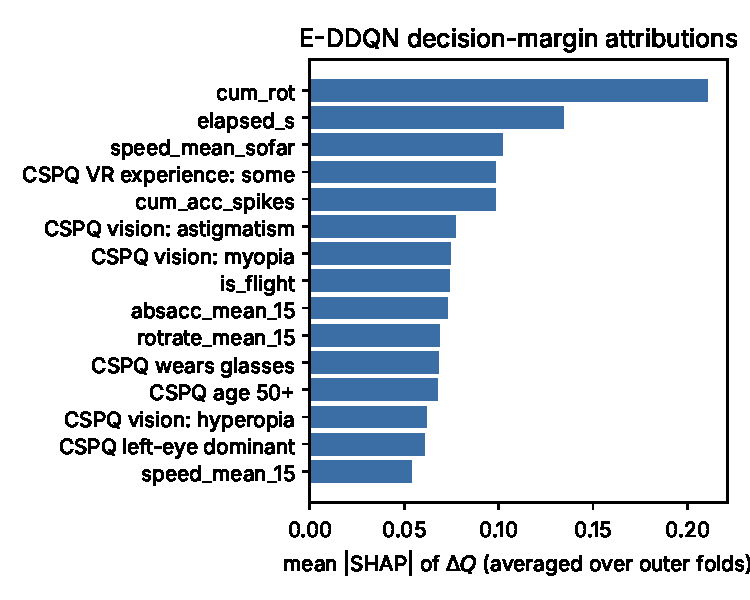
\includegraphics[width=0.92\columnwidth]{figs/shap_margin.pdf}
\caption{Mean absolute SHAP value of the E-DDQN decision margin $\Delta Q$, averaged over the five outer folds (one model per fold; attributions on that fold's test groups).}
\label{fig:shap}
\end{figure}
